\documentclass[11pt]{article}
\usepackage[top=20mm,bottom=30mm,left=20mm,right=20mm]{geometry}
\usepackage[utf8]{inputenc}
\usepackage{parskip}
\usepackage{abstract}

% Biblatex
\usepackage[block=space,bibencoding=utf8,style=phys,maxbibnames=6,giveninits=true]{biblatex}
\addbibresource{../StochasticTopology.bib}

% Mathy stuff
\usepackage{physics}
\usepackage{siunitx}
\usepackage{amsmath}
\usepackage[version=4]{mhchem}

% Visual stuff
\usepackage{graphics}
\usepackage{tikz}
\usetikzlibrary{math}
\usepackage{stackengine}
\usepackage{float}

% Misc
\usepackage{hyperref}
\usepackage{cleveref}
\usepackage{lipsum}

\renewcommand{\abstractname}{}    % clear the title
\renewcommand{\absnamepos}{empty} % originally center

\setlength{\parskip}{2ex}
\setlength{\parindent}{0em}

\begin{document}
\pagenumbering{gobble}
\begin{center}
	\LARGE
	\textbf{Topological States in Out-of-Equilibrium Allosteric Assemblies} \\
	\vspace{0.3em}
	\normalsize
	\textit{Jan Kocka}
	\vspace{1em}
\end{center}

\begin{abstract}
	\small
    \textit{
        I know this is too long (${\sim}260$ words), this is somewhat intentional so you can tell me what to cut out, in particular the "results" part is quite long and I don't love it and I need a more "zoomed-out" conclusion at the end.
        I also have some notes and questions for myself and you at the end which also includes what the format this is meant to be.
    }

	% General introduction to topology in biology/biophysics - 84 words
	Stochastic systems are key to many areas of biophysics as much of living matter takes place in a highly noisy environment.
	However, despite this noisiness, many biological systems show a high degree or robustness.
	A recent new direction in understanding this apparent paradox is the study of topology of stochastic systems\cite{tangTopologyProtectsChiral2021,soneHermitianNonHermitianTopology2024,zhengTopologicalMechanismRobust2024}.
	Topological states can effectively reduce the dimensionality of the configurational space and thus can explain robustness without making specific assumptions about the mechanics of a system, while themselves being robust to local changes.
	% Getting into the project - ~110 words
	In this study we look for topological features in a non-equilibrium, thermodynamically consistent stochastic model of an allosteric assembly where each unit can change conformation and (de)phosphorylate.
	The system is driven out of equilibrium by the inclusion of two different phosphorylation reactions: a direct reaction by (de)binding a phosphate group and one driven by ATP to ADP conversion.
	We allow these to couple differently depending on subunit conformation as this is to only way for an isolated subunit to favour undergoing a futile cycle of phosphorylating, changing conformation, dephosphorylating and changing conformation back.
	Such futile cycles are common in biological settings\cite{sharmaFutileCyclesEmerging2024,samoilovStochasticAmplificationSignaling2005} and give rise to topological currents when imposed artificially\cite{tangTopologyProtectsChiral2021}.
	% Getting on to results - 83
	We find that even without explicitly favouring futile cycles in the assembly, adding an energy cost to having a boundary between different conformations results in directed probability currents in the steady state.
    If both this energy cost and the ATP concentration are large then we get a connected current loop as in \cref{fig:loop} corresponding to the macroscale equivalent of the futile cycle.
    If either is reduced, this loops breaks in one place and the current is transferred along a diffuse network through the gap.

\end{abstract}

\vspace{1em}

\printbibliography

\vspace{1em}

\begin{figure}[H]
	\centering
	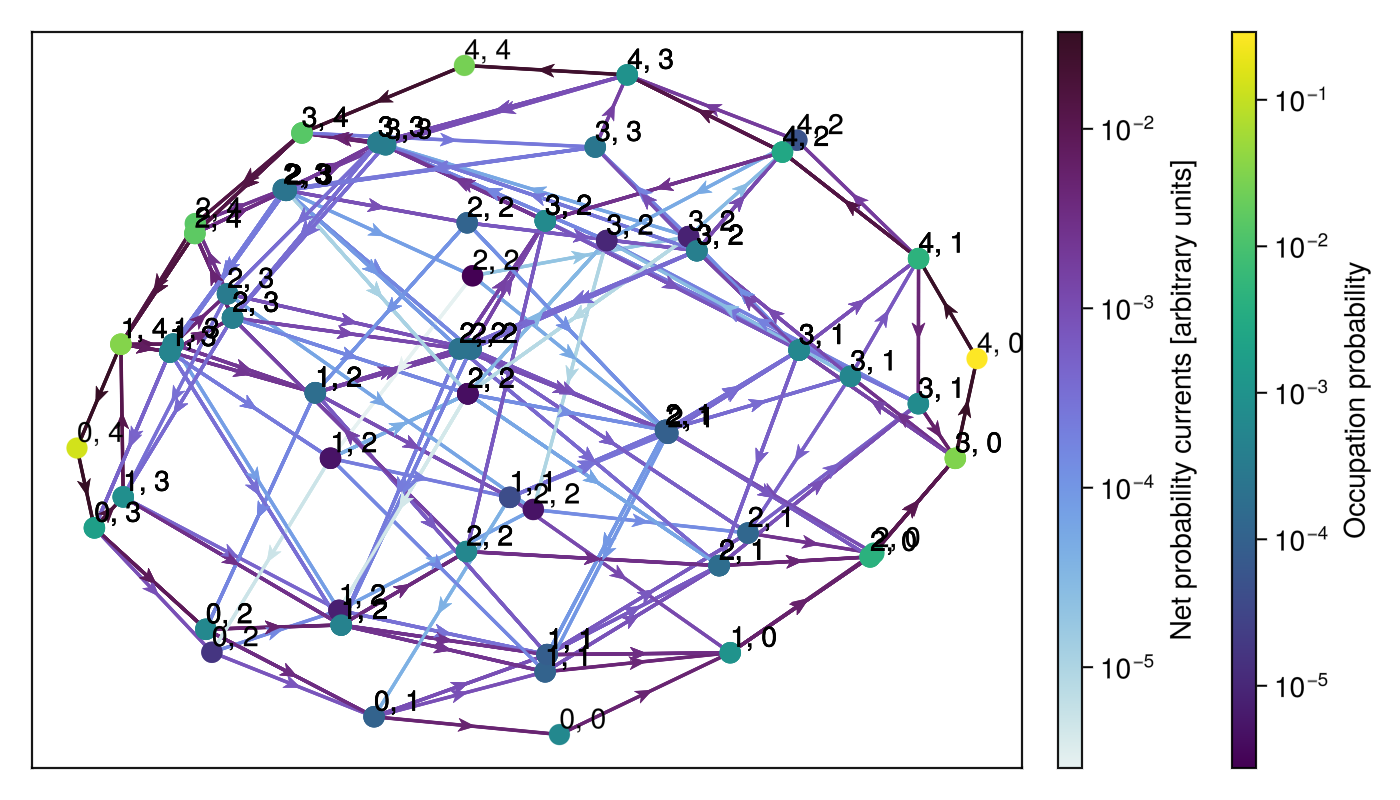
\includegraphics[width=\textwidth]{../../plots/aaa_B=1_C=2_N=4_version=2.5.png}
    \caption{
        Graph visualization of our system for a looped assembly of 4 subunits each of which can be in one of two conformations and bind up to one phosphate group.
        Subunits in conformation 1 are driven by ATP to bind a phosphate, subunits in conformation 2 are not and will unbind the phosphate (corresponding to high ATP and low ADP and P concentrations).
        Each node corresponds to a different microstate (though many are overlaid), their labels showing the number of bound ligands and the number of subunits in conformation 2.
        The node and edge colours correspond to the steady state probabilities of occupying a particular microstate and the corresponding net probability currents between them.
        This system is non-allosteric meaning all the substates of each monomer have the same energy, the only energy term in the model is an energy cost of $2\si{k}T$ per boundary between different conformations.
    }\label{fig:loop}
\end{figure}

\newpage
\section{Notes}
\paragraph{Format}
For POL2025 (the one due on the 6th) it should be 250 words, include references and up to 1 figure.
\paragraph{Topic}
I need to choose one of a list of topics.
Perhaps the closest might be: \textbf{"Biomolecular assemblies and condensates"} given that the main model is of an allosteric assembly?
Others that may be relevant:
\begin{itemize}
	\item "Patterns, waves, transport, collective phenomena, and microswimmers" -- there's collective phenomena! but idk about microswimmers
	\item "Clocks, timers and cell cycle dynamics" -- if we lean into KaiABC then maybe
	\item "Protein structure, dynamics and interactions" -- cause I guess the polymer as I've been calling it would realistically be a protein?
	\item "Emerging Areas in the Physics of Life" -- idk what this is but probably not
\end{itemize}

\subsection{Questions}
\begin{itemize}
	\item Approach to talk about a project that has only just started?
	\item Should I be talking about allostery or not so much? It seems relevant and as an interesting topic but it's not really a core ingredient in it.
    \item I'm a bit worried that the only "result" is a bit obvious once you think about it. If we add a penalty for NN having different conformation then of course the ones with all the same conformation will be preferred. Then if all are in conformation 1 (tense) then they are ATP driven to bind ligands so they do so. After that they are by our choice of parameters not favoured to debind hence the only thing they can do is change conformation. The same sort of reasoning then completes the cycle.
    \item Is an ArXiV citation admissible here?\cite{soneHermitianNonHermitianTopology2024}
\end{itemize}

\subsection{Key points to cover}
\begin{itemize}
	\item stochastic systems
	\item futile cycles
	\item non-equilibrium dynamics
	\item allostery
	\item system features
	      \begin{itemize}
		      \item complex -- high dimensional network, not pen-and-paper tractable
		      \item locality -- unlike the previous models, have NNs, can model waves along the polymer
		      \item discrete configurational space
		      \item Thermodynamically consistent? idk if this is the right wording
	      \end{itemize}
	\item Search for topological states/patterns in realistic systems (this means starting from the ground up with (non-equilibrium) statphys, LDB, no arbitrary choices) with futile cycles
	\item the futile cycle is implemented via physical parameters by coupling to two physically reasonable asymmetrical processes
\end{itemize}

% \subsection{"Formula"}
% \paragraph{Title/Topic}
% \paragraph{Motivation}
% Topological phases have been a hot topic in physics ever since the quantum hall effect.
% Recently their study has been extended to non-Hermitian systems such as a non-reciprocal stochastic processes.
% \paragraph{Problem}
% Idrk?
% \paragraph{Study design}
%
% \paragraph{Predictions and results}
% \paragraph{Conclusions}

\end{document}
